% !TEX TS-program = xelatex
% !TEX encoding = UTF-8 Unicode

% \documentclass[AutoFakeBold]{LZUThesis}
\documentclass[AutoFakeBold]{LZUThesis}

\begin{document}
%=====%
%
%封皮页填写内容
%
%=====%

% 标题样式 使用 \title{{}}; 使用时必须保证至少两个外侧括号
%  如: 短标题 \title{{第一行}},  
% 	      长标题 \title{{第一行}{第二行}}
%             超长标题\tiitle{{第一行}{...}{第N行}}

\title{{人类DNA指纹分析}}



% 标题样式 使用 \entitle{{}}; 使用时必须保证至少两个外侧括号
%  如: 短标题 \entitle{{First row}},  
% 	      长标题 \entitle{{First row}{ Second row}}
%             超长标题\entitle{{First row}{...}{ Next N row}}
% 注意:  英文标题多行时 需要在开头加个空格 防止摘要标题处英语单词粘连。
\entitle{{Human DNA Fingerprint Analysis}}

\author{生物信息学班 李泽华 320210928501}
\major{遗传学}
\advisor{王铭裕}
\college{生命科学学院}
\grade{2021级}



%\maketitle

%==============================%
% ↓ ↓ ↓ 诚信说明页 授权说明书
%==============================%

% 1. 可以调整签字的宽度,现在是40
% 2. 去掉raisebox的相关注释(注意上下大括号对应),可以改变-5那个数字调整签名和横线的上下位置

\mysignature{
    % \raisebox{-5pt}{
    
\includegraphics[width=40pt]{signature.pdf}
    % }
}
% 你手写的日期,signature.pdf 改为你的手写的日期文件名
\mytime{
    % \raisebox{-5pt}{
    
\includegraphics[width=40pt]{signature.pdf}
    % }
}
% 老师的手写签名,signature.pdf 改为老师的手写签名文件名
\supervisorsignature{
    % \raisebox{-5pt}{
    
\includegraphics[width=40pt]{signature.pdf}
    % }
}
% 老师手写的时间,signature.pdf 改为老师的手写的日期文件名
\teachertime{
    % \raisebox{-5pSt}{
    
\includegraphics[width=40pt]{signature.pdf}
    % }
}
% 老师手写的成绩
\recommendedgrade{
    % \raisebox{-5pt}{
    
\includegraphics[width=40pt]{signature.pdf}
    % }
}

%\makestatement

%==============================%
% ↑ ↑ ↑ 诚信说明页 授权说明书
%==============================%


%=====%
%论文(设计)成绩:注意2007的模板要求,成绩页在最后,2021要求成绩页在摘要前面
%=====%

%% 下面这些注释掉可以去掉成绩、评语什么的
%\supervisorcomment{导师评价你人很好}
%
%
%\committeecomment{优秀}
%
%\finalgrade{100}
%% 上面这些注释掉可以去掉成绩、评语什么的


\frontmatter



%中文摘要
\ZhAbstract{
    本研究聚焦于遗传标记和DNA指纹技术,深入探讨了遗传标记在遗传学和分子生物学领域的发展历程。特别关注DNA分子标记,其演变经历了形态标记、细胞学标记、生化标记和DNA分子标记四个阶段。DNA分子标记的核心是DNA指纹技术,通过该技术可以生成DNA指纹图谱,从而实现对生物个体或种群间基因组差异的分析。

人类DNA指纹分析成为研究重点,其中可变数目串联重复序列(VNTR)和短串联重复序列(STR)是主要关注对象。VNTR和STR在人类基因组DNA中展现高度多态性,通过PCR扩增和电泳检测等方法,可以获取有关基因型的信息。本实验选择了三个VNTR基因座(D1S80、D17\$30和ApoB3’)和四个21号染色体上的STR基因座(D21S11、D21S1432、D21S2054和D21S1446)进行研究。实验方法包括全血DNA提取、PCR扩增、电泳与检测以及数据记录与分析。

研究的目的在于深入了解DNA指纹分析技术的原理和应用,掌握可变数目串联重复序列和短串联重复序列多态性的检测和分析方法。通过实验,旨在了解串联重复序列多态性的含义,掌握相关技术操作,并为遗传学和分子生物学领域的研究提供实质性的数据支持。
}{遗传标记, DNA指纹技术, 可变数目串联重复序列(VNTR), 短串联重复序列(STR), PCR扩增, 电泳检测,人类DNA指纹分析, 实验方法, 多态性, Hardy-Weinberg平衡}


%英文摘要
\EnAbstract{
    This study delves into the field of genetic markers and DNA fingerprinting technology, tracing the evolutionary stages from morphological markers to DNA molecular markers. Emphasis is placed on DNA fingerprinting, a technique that generates DNA profiles reflecting genomic differences between individuals or populations.

Human DNA fingerprint analysis, with a focus on variable number tandem repeats (VNTR) and short tandem repeats (STR), is investigated. Three VNTR loci (D1S80, D17\$30, and ApoB3’) and four 21st chromosome STR loci (D21S11, D21S1432, D21S2054, and D21S1446) are selected for the experiment. Methods include whole blood DNA extraction, PCR amplification, gel electrophoresis, and data analysis.

The purpose of the study is to comprehensively understand the principles and applications of DNA fingerprint analysis, master the detection and analysis methods of variable number tandem repeats and short tandem repeats polymorphisms. The experiment aims to reveal the significance of tandem repeat polymorphism, provide hands-on experience in relevant techniques, and contribute substantial data support to the fields of genetics and molecular biology.

}{Genetic markers
, DNA fingerprinting technology
, Variable number tandem repeats (VNTR)
, Short tandem repeats (STR)
, PCR amplification
, Gel electrophoresis
, Human DNA fingerprint analysis
, Experimental methods
, Polymorphism
, Hardy-Weinberg equilibrium}

%生成目录
% \tableofcontents
% 下面这个包含图表目录
\customcontent


% % 部分同学需要专业术语注释表,* 表示不加入目录
% \chapter*{专业术语注释表}
% \begin{longtable}{lll}
%   \caption*{缩略词说明}\\
%   SS & Spread Spectrum & 扩展频谱 \\
%   PAPR & Peak to Average Power Ratio & 峰均比\\
%   DCSK & Differential Chaos Shift Keying &差分混移位键控\\
%   dasd & fdhfudw eqwrqw fasfasfs fewev wqfwefew &\tabincell{l}{太长了\\换行一下}\\
% \end{longtable}


%文章主体
\mainmatter
%TODO 包括研究背景、立论根据、研究内容、研究方法与过程、研究结果与分析、研究结论及其意义。

\chapter{\texorpdfstring{绪 \quad 论}{绪论}}
随着分子生物学和遗传学领域的飞速发展,遗传标记和DNA指纹技术成为研究基因组和个体差异的关键工具。遗传标记是在基因组中标识和检测特定基因或DNA区域的分子标记,其演变历程反映了科学技术的进步。DNA指纹技术作为遗传标记的一种重要形式,具有高度敏感性和准确性,广泛应用于法医学、人类学、亲权鉴定等领域。

遗传标记的发展经历了多个阶段,从形态标记、细胞学标记、生化标记到当前的DNA分子标记。DNA分子标记以其高效的分辨率和稳定性,逐渐取代了前几代标记方法,成为研究个体间基因组差异的主流手段。其中,DNA指纹技术通过生成DNA指纹图谱,展现了生物个体或种群之间的基因差异,成为遗传学研究的重要工具。

人类DNA指纹分析是DNA指纹技术的一个重要应用领域。可变数目串联重复序列(VNTR)和短串联重复序列(STR)是DNA指纹分析的核心内容,它们在人类基因组中呈现出丰富的多态性。本研究选择了具有代表性的VNTR和STR基因座,通过PCR扩增和电泳检测等技术手段,旨在深入了解串联重复序列多态性的含义,并掌握其检测和分析方法。

\chapter{研究背景}
\section{遗传标记和DNA指纹技术}
遗传标记在遗传学的建立和发展过程中有着举足轻重的作用,随着遗传学的进一步发展和分子生物学的异军突起,遗传标记先后相应地经历了形态标记、细胞学标记、生化标记和DNA分子标记四个发展阶段。DNA分子标记本质上是指能反映生物个体或种群间基因组中某种差异的特异性DNA片段。DNA分子标记大多以电泳谱带的形式表现生物个体之间的DNA差异,通常也称为DNA的指纹图谱。产生DNA指纹图谱的过程叫作DNA指纹分析。DNA指纹技术的发展日新月异,第一代的分子标记是以Southem 杂交为基础的限制性片段长度多态(restriction fragment length polymorphism,RFLP),第二代分子标记是以PCR\cite{saiki1985enzymatic}为基础的各种DNA 指纹标记,如RAPD、 AFLP、短串联重复序列(shorttandem repeats,STR)和可变数目的重复序列 (variable number of tandem repeat,VNTR),第三代分子标记是以单核苷酸多态性为基础的SNP。一种理想的分子标记应具有以下特点:多态性高,重复性和稳定性好,带型清晰,容易统计,在染色体上均匀分布,共显性,简单快速,易自动化,开发和使用成本低廉等。\par
\section{人类DNA指纹分析}
人类基因组DNA 中存在一类串联重复序列,其核心序列的长度为10~70bp,该串联重复单位(核心序列)数目在人群中存在较大差异,具有高度多态性,称为可变数目串联重复序列(VNTR)或小卫星(mini-satellite)DNA。短串联重复序列(STR)形成多态性的原理与VNTR 基本相同。STR的核心序列短,为2~7bp,片段长度为100~500bp。STR位点广泛地分布在人类基因组中。据估计,在人类基因组中,每20kb就有一个包含3或4个核苷酸重复序列的STR位点。因STR具有高度多态性及遗传稳定性,已逐渐取代RFLP、VNTR而被广泛应用于遗传疾病的诊断和法医学个人识别。\par
\section{基因座选择}
本实验选择人类基因组中的三个 VNTR 基因座(D1S80, D17\$30和ApoB3’)和21号染色体上的四个STR 基因座(D21S11,D21S1432,D21S2054和D21S1446)作为研究对象,通过对人基因组 DNA的提取、多态性片段的PCR扩增以及电泳检测,了解串联重复序列多态性的含义和原理,掌握其检测和分析方法。\par

\chapter{研究目的与方法}
\section{实验目的}
\begin{itemize}
    \item 了解DNA指纹分析技术的原理和应用。
    \item 级悉可發效国事联正复序3 YNTB)列知事联重复序列(SPR)多态性的含义。
    \item 掌握可变数目串联重复序列和短串联重复序列多态性的检测和分析方法。
\end{itemize}
\section{实验方法}

\subsection{实验材料与数据收集}
\begin{itemize}
    \item 实验数据\par
    参试者口腔上皮细胞
    \item 实验试剂\par
    \begin{enumerate}
        \item 口腔上皮细胞DNA 提取\par
        \begin{itemize}
            \item 0.4\%生理盐水。\par
            \item 裂解液:25 mmol/L NaOH,0.2 mmoI/L EDTA(乙二胺四乙酸)。\par
            \item Tris-HCI(40 mmol/L,pH 5.0)。\par
            \item 无水乙醇。\par
            \item TE: 7 10 mmol/L Tris-HCI (pH8.0) # 1 mmol/L EDTA.\par
        \end{itemize}
        \item 全血DNA提取\par
        \begin{itemize}
            \item 5\% Chelex100 溶液:\par
            \item Chelex 100 (Bio-Rad) 0.5 g, 50 mmol/L. Tris-HCI 10 \, \mu\text{L}, 用
            4 mol/LNaOH调pH至11.0,室温可保存3个月,使用前充分混匀。\par
        \end{itemize}
        \item PCR 试剂\par
        \begin{itemize}
            \item 2×Taq PCR Master Mix, ddIl.O,上下游引物,模板 DNA。\par
        \end{itemize}
        \item 电泳检测试剂
        \begin{itemize}
            \item 2.0\%琼脂糖凝胶:称取2.0g琼脂糖放人250 \, \mu\text{L}. 三角烧瓶,加入1XTAE 溶液100\, \mu\text{L} 微波炉加热溶解,冷却60\,^\circ\mathrm{C}$左右加入终浓度为1wg/\, \mu\text{L}.溴化乙锭(EB),缓慢混匀后倒胶板。\par
            \item 10×TAE电泳缓冲液:Tris 48.4g,冰醋酸11.42 \, \mu\text{L}, 0.5 mol/LEDTA (pH8.0) 20\, \mu\text{L},蒸馏水定容至1000 \, \mu\text{L},室温保存。\par
            \item 0.5 mo/L EDTA (pH8.0): Naz EDTA 18.61 g,NaOH 2.0g,蒸馏水定容至100\, \mu\text{L}。\par
            \item 溴化乙锭(EB):用无菌水配制5 mg/\, \mu\text{L}储藏液,工作浓度1 wg/ml。\par
            \item  10x上样缓冲液(Loading dye):溴酚蓝0.25g,二甲苯腈蓝0.25g,蔗糖50.0g(或甘油50\, \mu\text{L}),用无菌水60\, \mu\text{L}(用甘油时49\, \mu\text{L})溶解上述试剂,定至100\, \mu\text{L},室温保存。\par
            \item 0.16 mol/L硝酸溶液。\par
            \item  10 mmo/L硝酸银溶液。\par
            \item 0.28 mol/L碳酸钠溶液。\par
            \item 1.67 mol/L乙酸。\par
            \item 聚丙烯酰胺,DNA相对分子质量标记。\par
        \end{itemize}
    \end{enumerate}
    \item 实验仪器\par
    微量移液器、高速冷冻离心机、恒温水浴锅、旋涡振荡器、PCR扩增仪、电泳仪、电泳槽、凝胶成像系统、冰箱、制冰机、无菌枪头、无菌离心管(1.5 \, \mu\text{L},0.5 \, \mu\text{L})、无菌棉签、离心管盒、枪头盒、纸杯等。
\end{itemize}
\subsection{可变数目串联重复序列(VNTR)}
\begin{enumerate}
    \item 基因组DNA 的提取\par
    \begin{enumerate}
        \item 漱口,用无菌棉签刮取口腔脱落上皮细胞\par
        \item 将富集口腔脱落細胞的口監拭于放人盤有人m生和不的1.3\, \mu\text{L}离心管中。\par
        \item 将拭子置于振荡器上,振荡1min 左右,少心地娶這相金,再用适最的生理盐水冲洗。\par
        \item 13000rmin离心Jmin、小入批将主余的消被全部取起。记能物即为脱答上皮細胞,\par
        \item 在流淀中加人25~50ML裂解液,振満10s。\par
        \item 98と孵育20min,振満后加入等体根Tis-HICI (40 mmol/L, pH5.0)。\par
        \item 13 000 t/min 离心10 min,取上清液。\par
        \item 加入无水乙醇,$-20\,^\circ\mathrm{C}$放置15 min。\par
        \item 13000 r/min 离心15 mino\par
        \item 弃上清,晾干后即得到口腔脱落上皮细胞DNA。\par
        \item 加入适量TE 溶解 DNA,$4\,^\circ\mathrm{C}$或$-20\,^\circ\mathrm{C}$保存待用。\par
        为提高DNA的产率和纯度,可选用TANamp SwabDNA Kit(口腔拭子基因组DNA提取试剂盒,离心柱型,目录号:DP322)。\par
    \end{enumerate}
    \item PCR扩增\par
    3个VNTR基因座的引物序列和PCR扩增体系及扩增参数分别见表\ref{tab:table1}和表\ref{tab:table2}。\par
    \begin{longtable}{c|p{4.7cm}cccc}
        \toprule
        位点 & \centering{引物序列} & 変性 & 退火 & 延伸 & 循环数 \\
        \midrule
        Marker & Primer Sequences & \SI{95}{\degreeCelsius}, \SI{60}{\second} & \SI{65}{\degreeCelsius}, \SI{60}{\second} & \SI{72}{\degreeCelsius}, \SI{60}{\second} & Cycle \\
        DIS80 & \centering \tiny 5'-GAAACTGGCCTCCAAACACTGCCCGCCG-3'\par 5'-GTCTTGTTGGAGATGCACGTGCCCCTTGC-3' & \SI{95}{\degreeCelsius}, \SI{60}{\second} & \SI{65}{\degreeCelsius}, \SI{60}{\second} & \SI{72}{\degreeCelsius}, \SI{60}{\second} & 30 \\
        D17S30 & \centering \tiny 5'-GGAAGAGTGAAGTGCACAGG-3'\par 5'-CACAGTCTTTATTCTTCAGCG-3' & \SI{94}{\degreeCelsius}, \SI{30}{\second} & \SI{55}{\degreeCelsius}, \SI{30}{\second} & \SI{72}{\degreeCelsius}, \SI{80}{\second} & 30 \\
        ApoB3' & \centering \tiny 5'-ATGGAAACGGAGAAATTATG-3'\par 5'-CCTTCTCACTTGGCAAATAC-3' & \SI{94}{\degreeCelsius}, \SI{60}{\second} & \SI{63}{\degreeCelsius}, \SI{60}{\second} & \SI{72}{\degreeCelsius}, \SI{120}{\second} & 26 \\
        \bottomrule
        \caption{3个VNTR基因座的引物序列和PCR扩增条件}
        \label{tab:table1} \\
    \end{longtable}

    \begin{longtable}{cc}
        \toprule
        名称 & 体积/微升 \\
        \midrule
        上游引物(5wm) & 1.0 \\
        下游弓物(5wm) & 1.0 \\
        2xTaq PCR Master Mix & 12.5 \\
        dd$H_2O$ & 0.5 \\
        模板 DNA & 10.0 \\
        总体积 & 25.0 \\
        \bottomrule
        \caption{3个VNTR位点PCR扩增体系}
        \label{tab:table2} \\
    \end{longtable}

    \item 电泳与检测\par
    采用2\%琼脂糖凝胶60V电泳,30~40 min后取出凝胶用清水漂洗5~10 min。凝胶成像系统观察和记录每个个体的DNA条带数目及其位置\par
    \item 数据记录与分析\par
    读取各个体样本的基因型,计算基因型频率及等位基因频率,用x检验进行Hardy-Neinberg 平衡吻合度检验。\par
\end{enumerate}
\subsection{短串联重复序列(STR)}
\begin{enumerate}
    \item 基因组DNA的提取
    \begin{enumerate}
        \item 取 \SIrange{3}{10}{\milli\liter} 全血加入 \SI{1.5}{\milli\liter} 离心管中,再加入 \SI{500}{\micro\liter} 纯水,剧烈振荡,室温下放置 \SI{15}{\minute}。
        \item \SI{13000}{rpm} 离心 \SI{3}{\minute},弃去上清,收集沉淀。若需要,可使用蒸馏水反复清洗沉淀物,直至无色或血色素很少。
        \item 沉淀中加入 \SI{200}{\micro\liter} \SI{5}{\percent} Chelex-100溶液(\SI{5}{\percent} Chelex-100为悬浊液,使用前要充分振摇,使Chelex-100颗粒悬浮),在振荡器上反复振荡后,放入 \SI{56}{\degreeCelsius} 水浴保温 \SI{30}{\minute} 以上。
        \item 取出后振荡,\SI{100}{\degreeCelsius} 保温 \SI{8}{\minute},再振荡后,\SI{13000}{rpm} 离心 \SI{3}{\minute},上清用于PCR扩增,或放入 \SI{4}{\degreeCelsius} 保存备用。此DNA样本可在 \SI{4}{\degreeCelsius} 或 \SI{-20}{\degreeCelsius} 保存,必要时在使用前再次加热并离心,使管内物质分层。
    \end{enumerate}
    \item 位点选择及其特性(表\ref{tab:table3})\par
    \begin{longtable}{cccc}
        位点 & 重复序列 & 片段大小(bp) & 染色体位置(Mb) \\
        \midrule
        D21S11 & TCTG & 202-260 & 21q22.11 \\
        D21S1432 & ATAG/TAGA & 127-155 & 21q22.2 \\
        D21S2054 & TCTA & 162-182 & 21q22.11 \\
        D21S1446 & TCTA/ATCT & 160-187 & 21q22.3 \\
        \bottomrule
        \caption{4个21号染色体STR位点的基本参数}
        \label{tab:table3} \\
    \end{longtable}
    \item PCR扩增\par
    3个VNTR基因座的引物序列和PCR扩增体系及扩增参数分别见表\ref{tab:table4}和表\ref{tab:table5}。\par
    \begin{longtable}{c|p{4.7cm}cccc}
        \toprule
        位点 & \centering{引物序列} & 変性 & 退火 & 延伸 & 循环数 \\
        \midrule
        D21S11 & \tiny \centering 5'-TATGTGAGTCAATTCCCCAAG-3'\par 5' -GTTGTATTAGTCAATGTTCTCC-3' & \SI{95}{\degreeCelsius},15s & \SI{58}{\degreeCelsius},60s & \SI{60}{\degreeCelsius},60s & 30 \\
        D21S1432 & \tiny \centering 5'-CTTAGAGGGACAGAACTAATAGGC-3'\par 5'-AGCCTATTGTGGGTTTGTGA-3' & \SI{95}{\degreeCelsius},15s & \SI{60}{\degreeCelsius},60s & \SI{60}{\degreeCelsius},60s & 30 \\
        D21S2054 & \tiny \centering 5'-GAGTAAATGTCATGAAACAAGG-3'\par 5'-ATGATAGGTAGATGGATCAATTggAGA-3' & \SI{95}{\degreeCelsius},40s & \SI{56}{\degreeCelsius},40s & \SI{72}{\degreeCelsius},30s & 32 \\
        D21S1446 & \tiny \centering 5'-ATGTACGATACGTAATACTTGAGAA-3'\par 5'-GTCCCAAAGGACCTGCTC-3' & \SI{94}{\degreeCelsius},40s & \SI{56}{\degreeCelsius},50s & \SI{72}{\degreeCelsius},50s & 35 \\
        \bottomrule
        \caption{4个VNTR基因座的引物序列和PCR扩增条件}
        \label{tab:table4} \\
    \end{longtable}
    \begin{longtable}{cc}
        \toprule
        名称 & 体积/微升 \\
        \midrule
        上游引物(S wm) & 2.2 \\
        下游引物(S wm) & 1.2 \\
        2XTaq PCR MasterMix & 6.0 \\
        dd$H_2O$ & 2.1 \\
        模板DNA & 2.0 \\
        总体积 & 12.5 \\
        \bottomrule
        \caption{4个21号染色体STR位点PCR扩增体系}
        \label{tab:table5} \\
    \end{longtable}
    \item 变性凝胶电泳 \\
    取扩增产物 2.0μL 与 2.0μL 变性加样缓冲液混合均匀,\SI{95}{\degreeCelsius} 变性 \SI{2}{\minute},立即置于冰浴,采用 \SI{6}{\percent} 变性聚丙烯酰胺凝胶垂直电泳,先预电泳 \SI{1}{\hour},上样后恒功率 \SI{40}{\watt},电泳 \SI{3}{\hour}。完毕后将凝胶取下,用双蒸水冲洗1次,置于 \SI{0.16}{\molar} 氮酸溶液中,轻摇反应 \SI{10}{\minute},双蒸水冲洗,再置于 \SI{10}{\milli\molar} 氮酸银溶液中,轻摇反应 \SI{20}{\minute},双蒸水冲洗,然后置于 \SI{0.28}{\molar} 碳酸钠溶液中,轻摇反应,至条带清晰后加入 1.67 \mu\text{L 乙酸终止反应并固定显色。}
    
    \item DNA序列的测定 \\
    挑选每个SIR位点中至少2个以上不同片段长度的纯合子样本,经PCR扩增及纯化试剂盒纯化后进行DNA序列测定,根据测序结果推测其余不同片段长度等位基因的重复数。
    
    \item 统计学分析 \\
    运用直接计数法观察位点的基因频率,通过PowerStats软件进行数据统计分析,计算杂合度(heterozygosity,H)、多态信息量(polymorphism information content, PIC)及个体识别率(average power of discrimination, PD)。用 $\chi^2$ 进行 Hardy-Weinberg平衡吻合度检验。

    $$
    H = 1 - \sum_{i=1}^{n}p_i^2
    $$
    其中: n为等位基因的数目, $p_i$为单位基因的频率。\par
    $$
    PIC = 1 - \sum_{i=1}^{n}p_i^2 - \sum_{i-1}^{n-1}\sum_{j=i+1}^{n}2p_i^2p_j^2
    $$
    其中: n为等位基因的数目, $p_i$为第一个等位基因在群体中的频率。\par

\end{enumerate}


\chapter{研究结果与分析}

\section{电泳结果}
在我们的实验中,21级生科院的同学们对基因进行了分析并得到了多个结果。其中,图 \ref{fig:anamainegimg} 展示了其中两组数据使用Gelanalysis分析后的分布情况, 这两个图具有代表性。

\begin{figure}[H]
    \centering

    \subfloat[dataimg2-1]{
        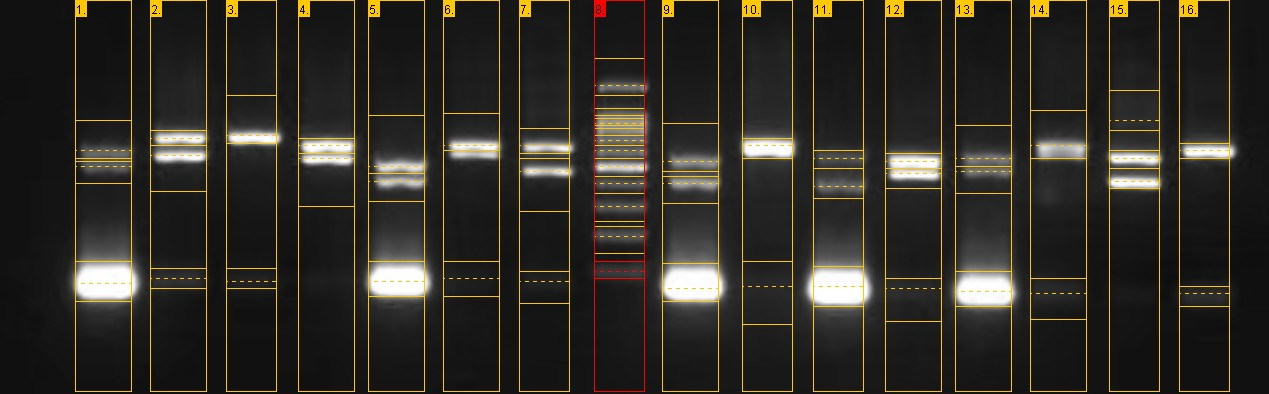
\includegraphics[width=0.4\textwidth]{data/ana_img2-1.jpg}
        \label{fig:anaegimg1}
    }
    \hfill
    \subfloat[dataimg2-2]{
        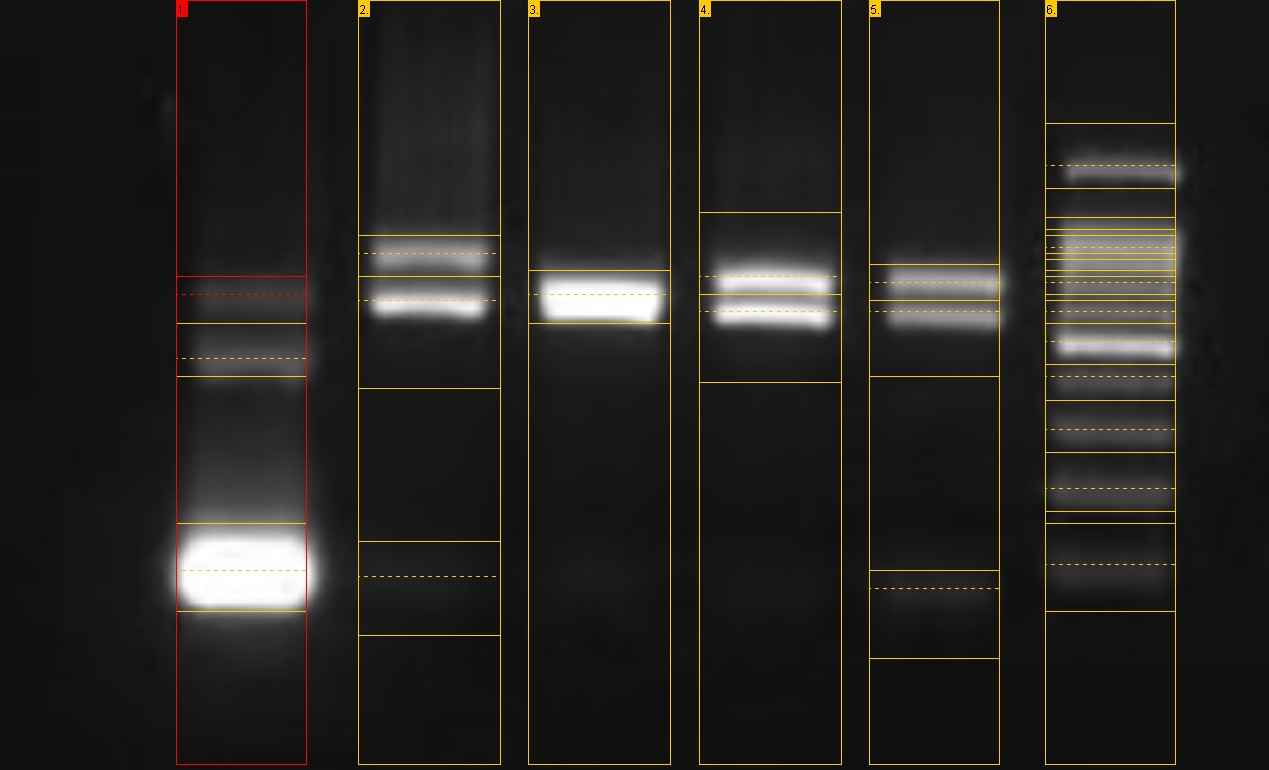
\includegraphics[width=0.4\textwidth]{data/ana_img2-2.jpg}
        \label{fig:anaegimg2}
    }
    \caption{电泳分析结果}
    \label{fig:anamainegimg}
\end{figure}

如图\ref{fig:anaegimg1}所示,我们可以看到,第八条跑道为marker有11条带(从上到下分别为: 1500bp, 1000bp, 900bp, ..., 100bp),
其余跑到均为样本, 大多样本有2个条带, 代表该样本为杂合子, 有两个等位基因, 也有少数样本只有一个条带, 代表该样本为纯合子, 只有一个等位基因。

图\ref{fig:anaegimg2}类似, 只是数据量较少, 且第六条跑道为marker.

由于实验涉及多组数据,其他的一些结果图被在附录中供读者参考。
\section{电泳条带数据}
我们使用Gelanalysis对电泳结果进行分析,得到了每个样本的电泳条带数据,表\ref{tab:anadataeg}展示了图\ref{fig:anaegimg2}中的各个条带数据。

\begin{longtable}{ccccccc}
    \hline
    Lane \# & Band \# & Peak Rf & Peak value & Raw volume & Cal. volume & MW \\
    \hline
    \endhead
    1 & 1 & 0.382 & 52 & 405 & - & 663 \\
    1 & 2 & 0.466 & 74 & 560 & - & 441 \\
    1 & 3 & 0.741 & 251 & 3355 & - & 114 \\
    2 & 1 & 0.329 & 129 & 763 & - & 859 \\
    2 & 2 & 0.39 & 187 & 1281 & - & 639 \\
    2 & 3 & 0.749 & 28 & 410 & - & 110 \\
    3 & 1 & 0.382 & 218 & 1704 & - & 663 \\
    4 & 1 & 0.359 & 196 & 1316 & - & 741 \\
    4 & 2 & 0.405 & 203 & 1226 & - & 593 \\
    5 & 1 & 0.367 & 144 & 767 & - & 714 \\
    5 & 2 & 0.405 & 132 & 804 & - & 593 \\
    5 & 3 & 0.764 & 34 & 376 & - & 102 \\
    6 & 1 & 0.214 & 96 & 592 & - & 1500 \\
    6 & 2 & 0.298 & 103 & 255 & - & 1000 \\
    6 & 3 & 0.321 & 140 & 517 & - & 900 \\
    6 & 4 & 0.336 & 125 & 352 & - & 800 \\
    6 & 5 & 0.367 & 102 & 370 & - & 700 \\
    6 & 6 & 0.405 & 98 & 422 & - & 600 \\
    6 & 7 & 0.443 & 178 & 869 & - & 500 \\
    6 & 8 & 0.489 & 70 & 379 & - & 400 \\
    6 & 9 & 0.558 & 68 & 470 & - & 300 \\
    6 & 10 & 0.634 & 62 & 474 & - & 200 \\
    6 & 11 & 0.733 & 43 & 449 & - & 100 \\
    \hline
    \caption{电泳条带数据}
    \label{tab:anadataeg} \\
\end{longtable}

可以看到跑道六有11个条带, 为marker与图\ref{fig:anaegimg2}中的第六条跑道对应, 而其他跑道有1-3个条带, 对应的MW为通过Gelanalysis计算得到的分子量, 其中小于177的条带都被认为是噪声, 将在数据处理中被过滤掉。

其他的数据结果请见附件

\section{数据处理与分析}
\begin{enumerate}
    \item 批量导入数据\par
    如代码\ref{lst:importdata}, 导入../data/目录下summary.csv以外的所有.csv文件, 并将其存储在data\_list中, data\_list中的每个元素都是一个pandas.DataFrame对象, 代表一个.csv文件的数据
    \begin{lstlisting}[language=python, caption={批量导入数据}, label={lst:importdata}, style=myPythonStyle]
import os
import pandas as pd

# 设置工作目录
os.chdir("F://Onedrive//study//生物//遗传学//实验报告//3_人类DNA指纹分析//python")

# 导入数据 ###########################
csv_files = [file for file in os.listdir("..\data") if file.endswith(".csv") and file != "summary.csv"]
csv_files = [os.path.join("..\data", file) for file in csv_files]
data_list = [pd.read_csv(file) for file in csv_files]
# 显示导入的数据 ######################
#for i, data in enumerate(data_list):
#    print(f"Data from file {csv_files[i]}:\n")
#    print(data)
    \end{lstlisting}

    \item 封装并清洗数据\par
    如代码\ref{lst:cleandata}, 将每个炮到数据清洗封装为一个Lane对象, 并将所有Lane对象存储在lane\_objects中, lane\_objects中的每个元素都是一个Lane对象, 代表一个泳道的数据
    \begin{lstlisting}[language=python, caption={封装并清洗数据}, label={lst:cleandata}, style=myPythonStyle]
    
    设定m_edge = 177, 代表电泳图谱中的噪声边界, 小于177的条带都被认为是噪声, 将在数据处理中被过滤掉
class DnaFingerprintLane:
"""
DNA 指纹泳道类
"""
def __init__(self, data, filename):
    self.m_filename = filename
    self.m_data = data
    
    self.m_edge = 177
    self.m_laneID = data["Lane #"].iloc[0]
    if len(data[" Band #"]) == 11:
        self.m_category = "marker"
        self.m_MW = None
        self.m_repeatNum = None
        self.m_homoORheter = None
    
    else:
        self.m_category = "sample"
        self.m_MW = data[" MW"][data[" MW"] > self.m_edge].astype(float).tolist()
        self.m_repeatNum = self.calculate_repeat_num()
        if len(self.m_MW) == 1:
            self.m_homoORheter = "homo"
        elif len(self.m_MW) == 2:
            self.m_homoORheter = "heter"
        elif len(self.m_MW) > 2:
            self.m_homoORheter = "contamination"
        elif len(self.m_MW) == 0:
            self.m_homoORheter = "no result"
        else:
            self.m_homoORheter = "???"
    
lane_objects = []

for i, data_frame in enumerate(data_list):
    for j in data_frame["Lane #"].unique():
        lane = data_frame[data_frame["Lane #"] == j]
        #DnaFingerprintLane(lane, csv_files[i]).printLane()
        lane_objects.append(DnaFingerprintLane(lane, csv_files[i]))
    \end{lstlisting}

    \item 计算重复数\par
    定义类方法calculate\_repeat\_num, 用于计算重复数, 代码\ref{lst:calc_repeat_num}

    \begin{lstlisting}[language=python, caption={计算重复数}, label={lst:calc_repeat_num}, style=myPythonStyle]    
def calculate_repeat_num(self):
    mw_series = pd.Series(self.m_MW)
    repeat_num = 1 + (mw_series[mw_series > self.m_edge] - 161) / 16
    return repeat_num.astype(float).tolist()
    \end{lstlisting}
    
    \item 数据可视化与保存\par
    将数据整理, 剔除没有数据与数据被污染的通道, 按照重复数的相似度进行排序, 并进行简单的可视化, 保存可视化结果, 数据保存到../data/summary.csv中, 具体代码见附录.

    \begin{itemize}
        \item 最终整理后的部分数据(表\ref{tab:finaldata}), 以及数据汇总(表\ref{tab:finalcount})

        \begin{longtable}{ccccc}
            \hline
            File & Lane & MW & RepeatNum & HomoOrHeter \\
            \hline
            \endhead
            ..\data\data10-1.csv & 16 & [468.0, 419.0] & [20.1875, 17.125] & heter \\
            ..\data\data7-2.csv & 11 & [472.0] & [20.4375] & homo \\
            ..\data\data10-2.csv & 8 & [472.0, 403.0] & [20.4375, 16.125] &heter \\
            ..\data\data8-1.csv & 8 & [476.0, 376.0] & [20.6875, 14.4375] & heter \\
            ..\data\data7-2.csv & 8 & [482.0] & [21.0625] & homo \\
            ..\data\data8-1.csv & 3 & [485.0] & [21.25] & homo \\
            ... & ... & ... & ... & ...\\
            \hline
            \label{tab:finaldata}
            \caption{整理后部分数据}
        \end{longtable}

        \begin{longtable}{cc}
            \hline
            type & num \\
            \hline
            \endhead
            heter & 106 \\
            homo  &  82 \\
            \hline
            \label{tab:finalcount}
            \caption{数据统计}
        \end{longtable}
        杂合率: 0.56383

        \item 可视化结果, 图\ref{fig:finalimg}
        \begin{figure}[H]
            \centering
        
            \subfloat[Row1-46]{
                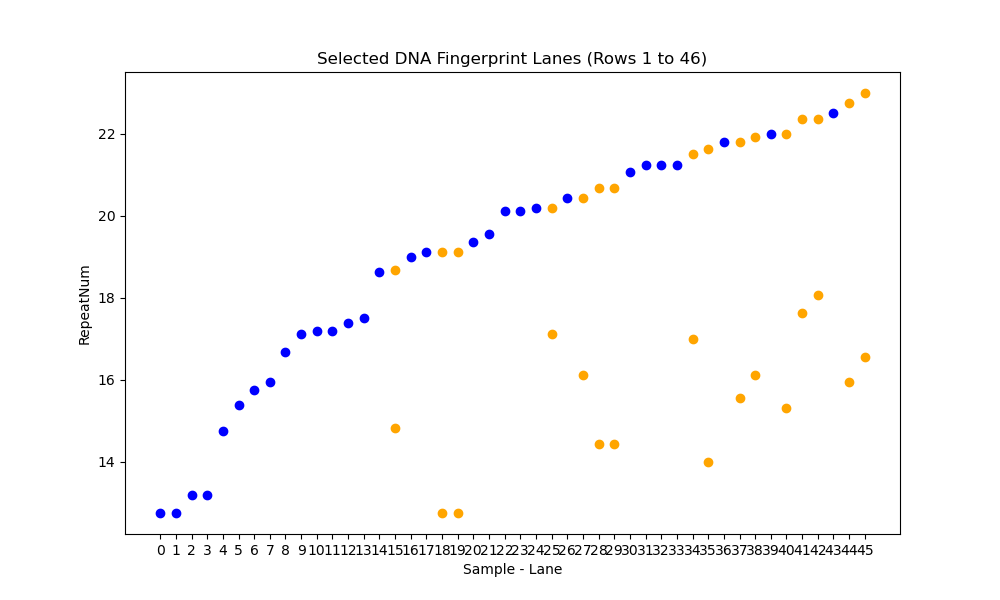
\includegraphics[width=0.45\textwidth]{output/result1.png}
                \label{fig:final1}
            }
            \hfill
            \subfloat[Row47-90]{
                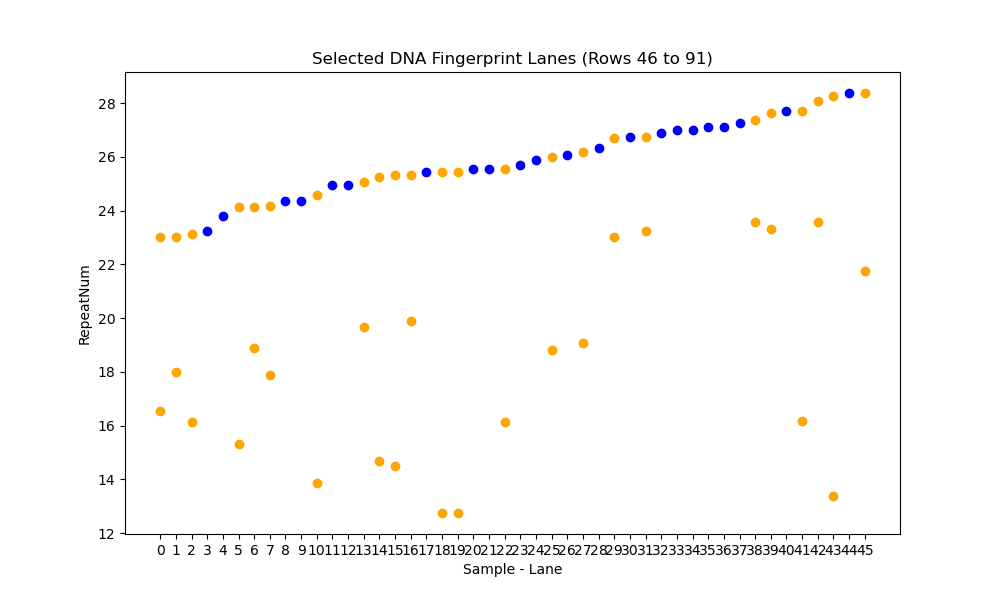
\includegraphics[width=0.45\textwidth]{output/result2.png}
                \label{fig:final2}
            }
            \hfill
            \subfloat[Row91-136]{
                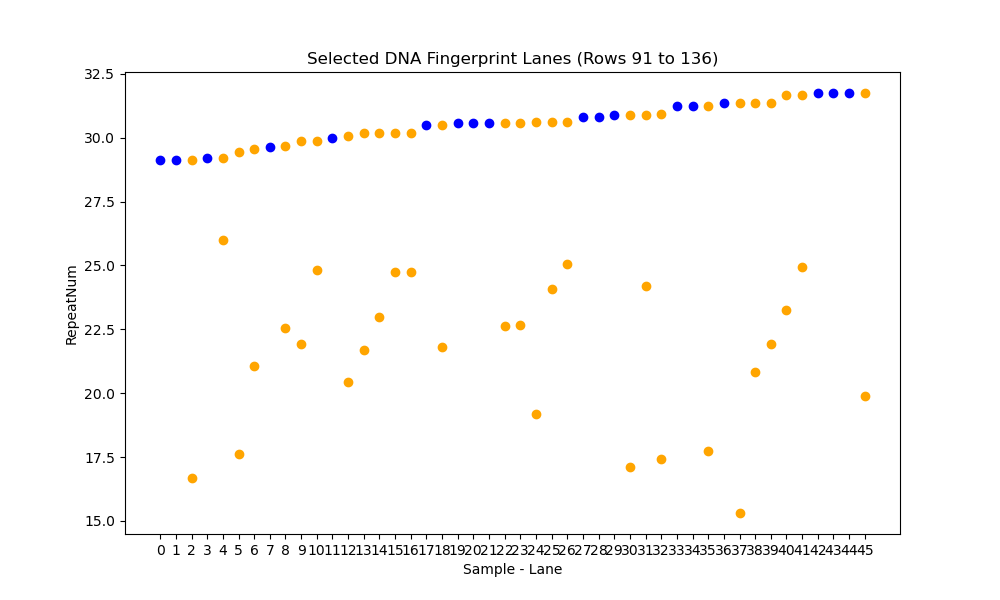
\includegraphics[width=0.45\textwidth]{output/result3.png}
                \label{fig:final3}
            }
            \hfill
            \subfloat[Row137-181]{
                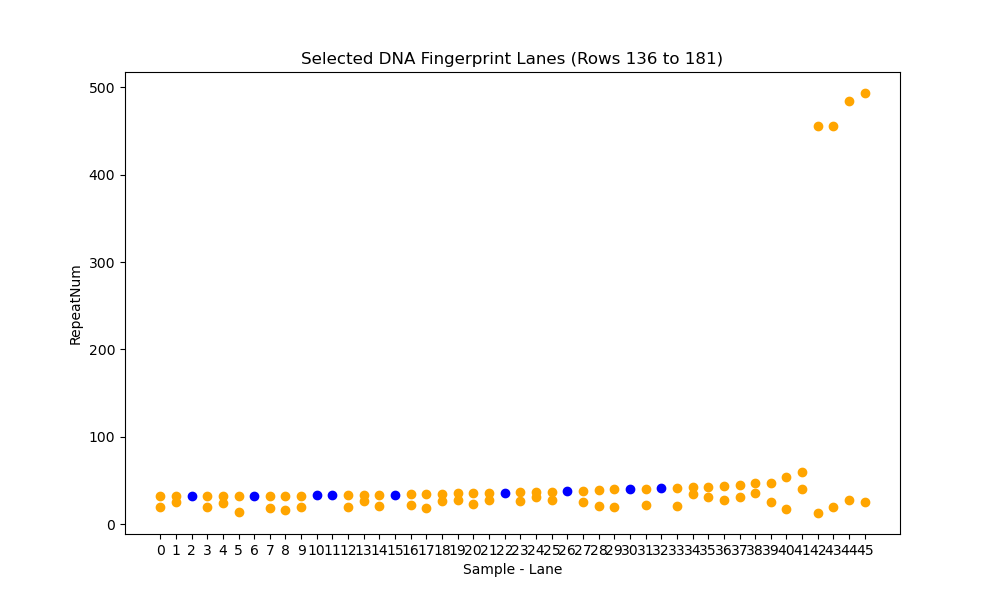
\includegraphics[width=0.45\textwidth]{output/result4.png}
                \label{fig:final4}
            }
            \hfill
            \subfloat[分布直方图]{
                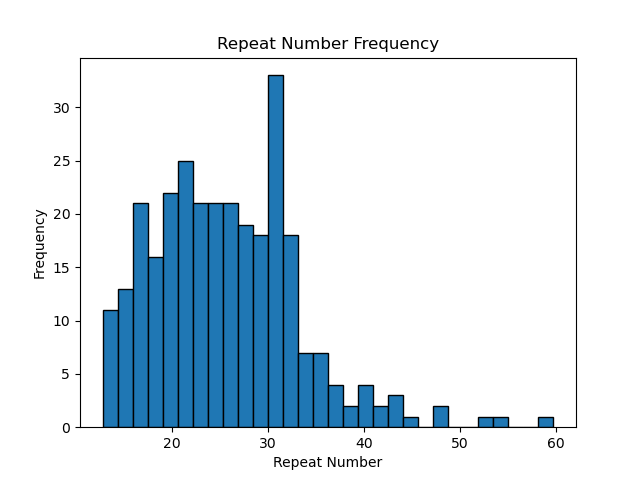
\includegraphics[width=0.5\textwidth]{output/frequencyimg.png}
                \label{fig:final5}
            }
            \caption{可视化结果}
            \label{fig:finalimg}
        \end{figure}

    \end{itemize}
\end{enumerate}


\chapter{\texorpdfstring{讨 \quad 论}{讨论}}

综上所述,我们通过实验成功进行了人类DNA指纹分析,主要关注可变数目串联重复序列(VNTR)和短串联重复序列(STR)的基因座。通过PCR扩增和电泳检测等技术手段,我们获得了电泳结果,并通过数据处理和分析,得到了每个样本的电泳条带数据。接着,我们进行了数据的清洗、封装、计算重复数以及最终的整理和可视化。

在数据处理的过程中,我们对电泳图谱中的噪声进行了边界设定,并清理了没有数据或被污染的通道。通过计算重复数,我们对样本的等位基因进行了分析,判断样本是纯合子还是杂合子。最终,我们将整理后的数据进行了可视化,并保存了数据汇总结果。

通过对103个杂合样本和78个纯合样本的统计,我们得到了杂合率为0.564。这些结果对于深入了解DNA指纹分析技术的原理和应用,以及掌握可变数目串联重复序列和短串联重复序列多态性的检测和分析方法具有重要意义。

但是这一结果与我们取其的结果相差较大,
我们认为这一结果的原因有以下几点:

\begin{enumerate}
\item 样本数量不足: 实验中选择了一部分样本进行分析,但样本数量相对较少,这可能限制了结果的普适性和可靠性。在今后的研究中,可以考虑增加样本数量,以更全面地了解DNA指纹分析的特征。

\item 数据的一致性: 在电泳结果中,有时出现了不同样本之间数据的一致性问题,例如重复数的计算可能存在一些差异。这可能是由实验操作中的技术差异或误差引起的。在未来的实验中,需要进一步优化实验步骤,提高数据的一致性。

\item 标准化处理: 在数据处理和分析过程中,可能存在一些标准化处理上的不足。例如,对于重复数的计算可能需要更加严格的标准和算法,以确保结果的准确性和可比性。

\item 深层次的统计分析: 对于得到的数据,我们进行了一些简单的统计分析,但在深层次的数据挖掘和统计学分析方面,仍有提升空间。可以探索更多的统计学方法,了解不同基因座之间的关系,进一步挖掘数据背后的信息。

\item 实验技术的进一步改进: 实验中使用的技术,如PCR扩增和电泳检测,是关键的步骤。技术水平的提高可能会改善实验结果的质量。在今后的实验中,可以考虑引入新的技术或改进现有技术,以提高实验的灵敏度和准确性。
\end{enumerate}

%论文后部
\backmatter


%=======%
%引入参考文献文件
%=======%
\bibdatabase{bib/database}%bib文件名称 仅修改bib/ 后部分
\printbib
\nocite{*} %显示数据库中有的,但是正文没有引用的文献



\Appendix

\section{电泳结果}

\begin{figure}[H]
    \centering

    \subfloat[dataimg1-1]{
        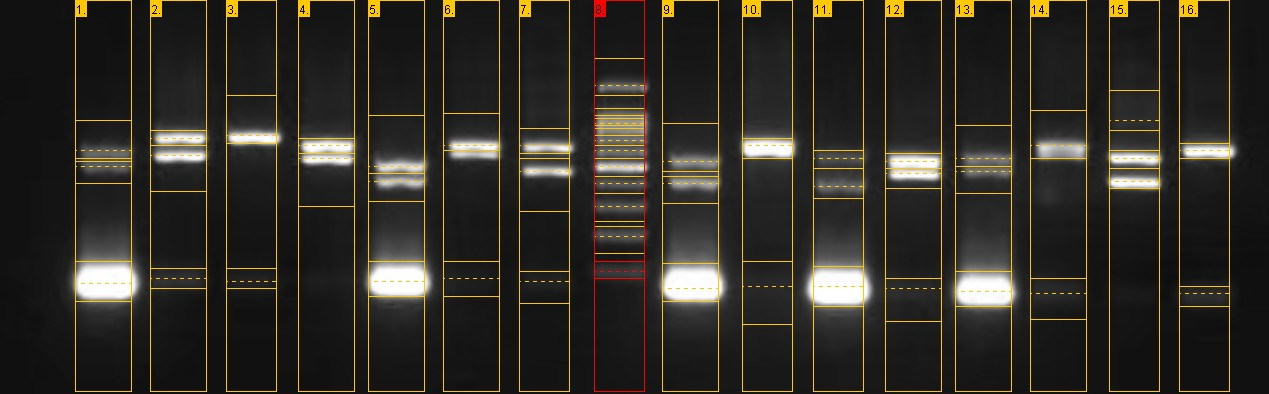
\includegraphics[width=0.4\textwidth]{data/ana_img2-1.jpg}
        \label{fig:anaegimg1}
    }
    \hfill
    \subfloat[dataimg1-2]{
        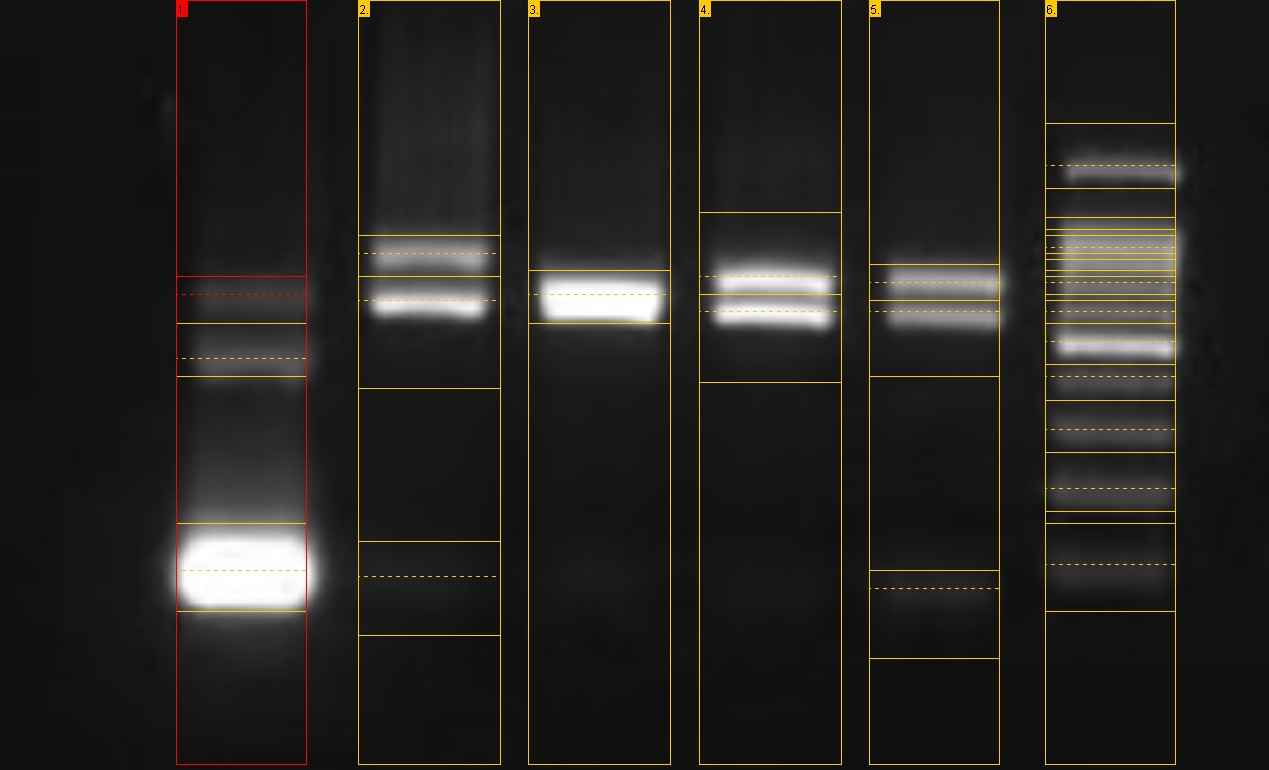
\includegraphics[width=0.4\textwidth]{data/ana_img2-2.jpg}
        \label{fig:anaegimg2}
    }
    \hfill
    \subfloat[dataimg1-3]{
        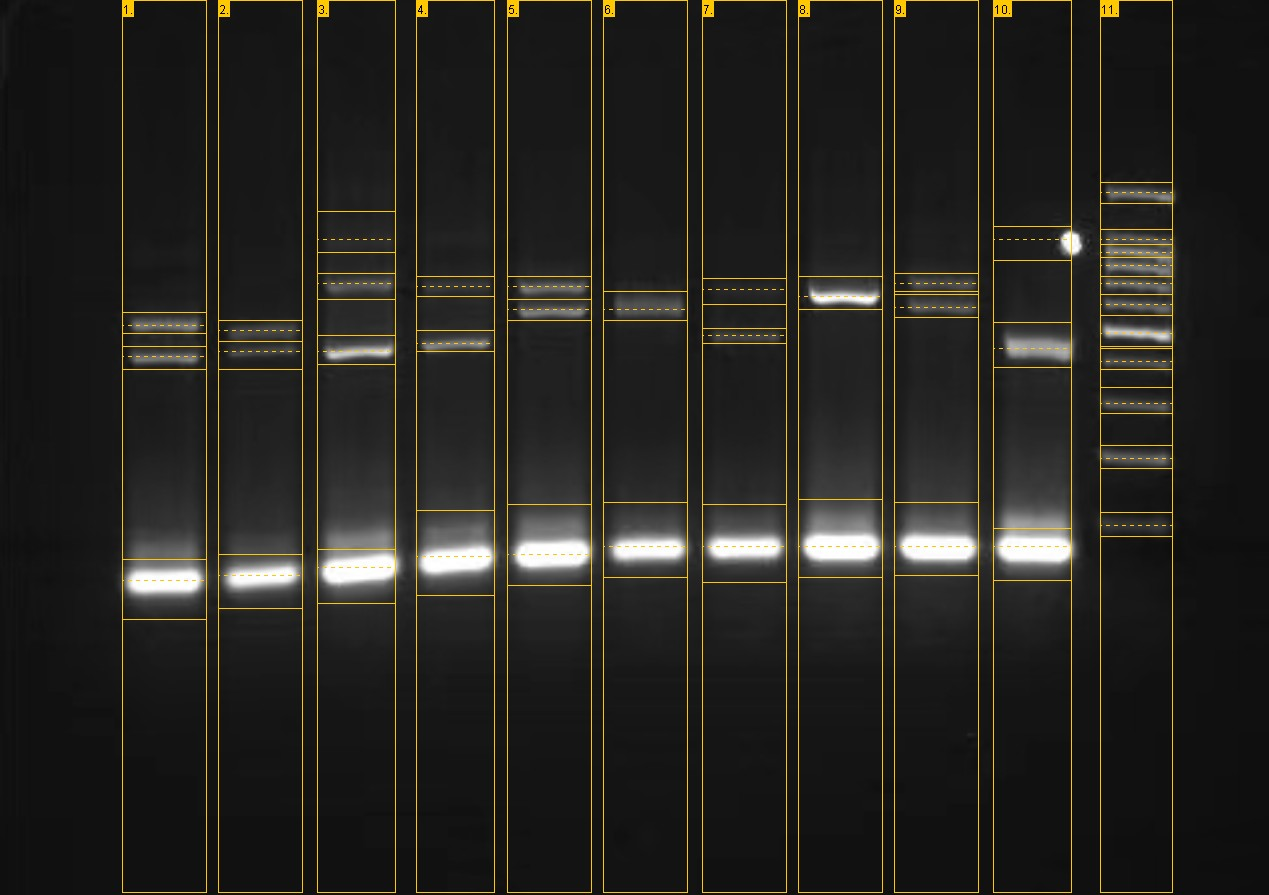
\includegraphics[width=0.4\textwidth]{data/ana_img3-1.jpg}
        \label{fig:anaegimg3}
    }
    \hfill
    \subfloat[dataimg1-4]{
        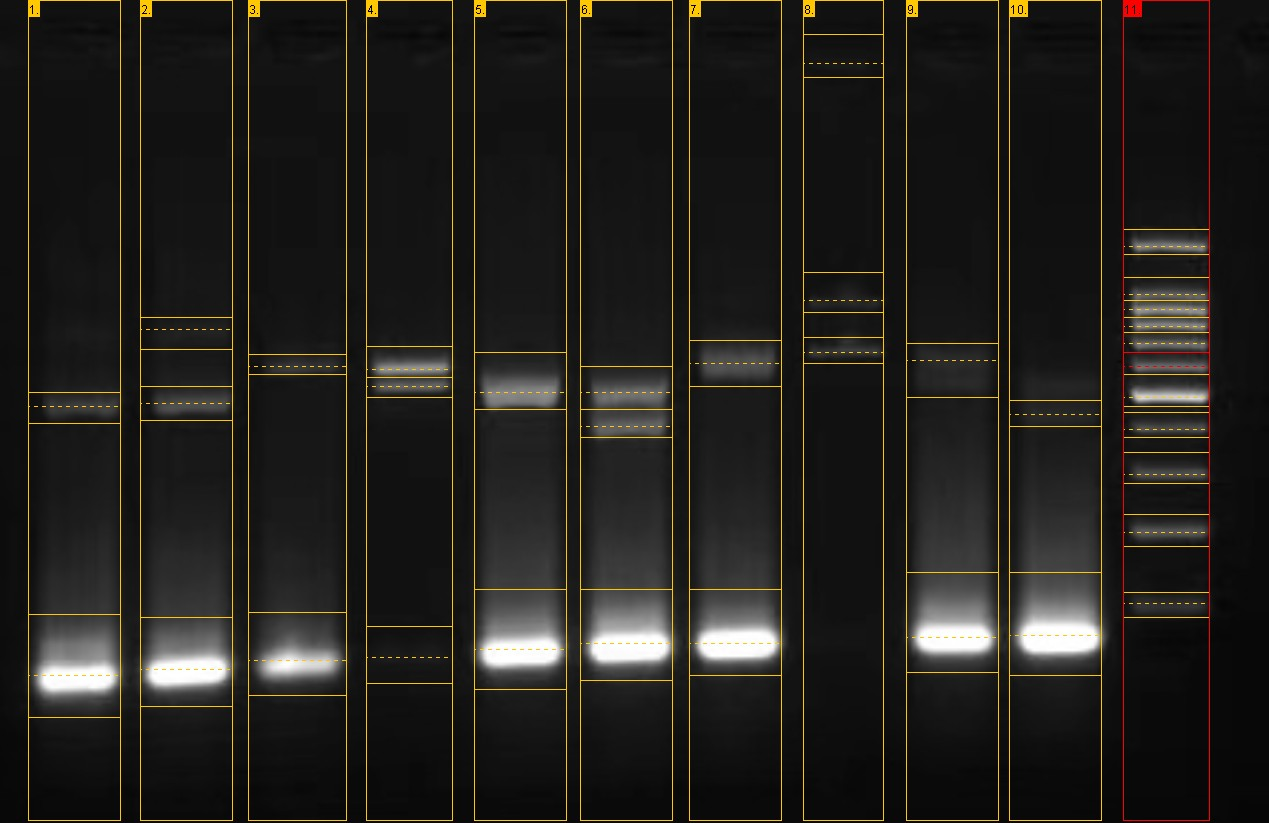
\includegraphics[width=0.4\textwidth]{data/ana_img3-2.jpg}
        \label{fig:anaegimg4}
    }
    \hfill
    \subfloat[dataimg1-5]{
        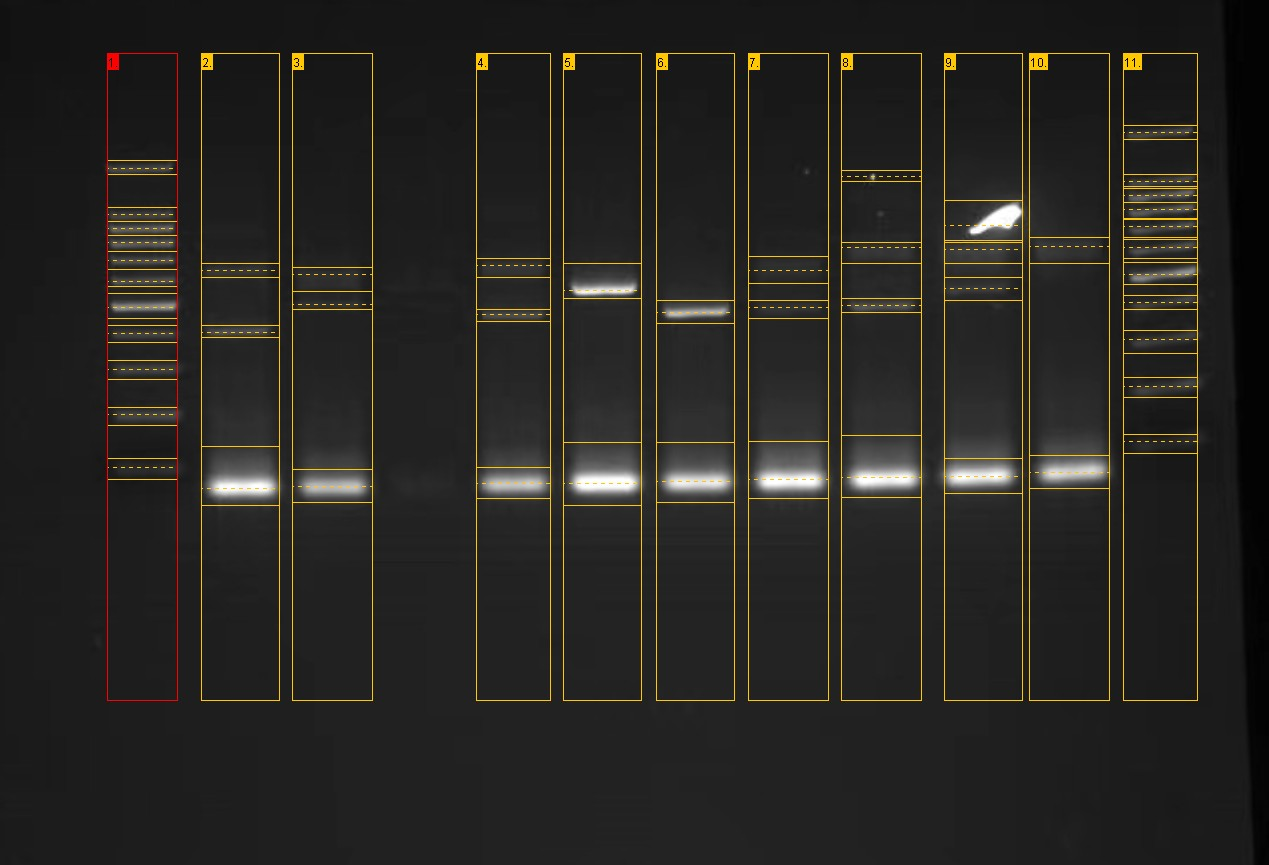
\includegraphics[width=0.4\textwidth]{data/ana_img4-1.jpg}
        \label{fig:anaegimg5}
    }
    \hfill
    \subfloat[dataimg1-6]{
        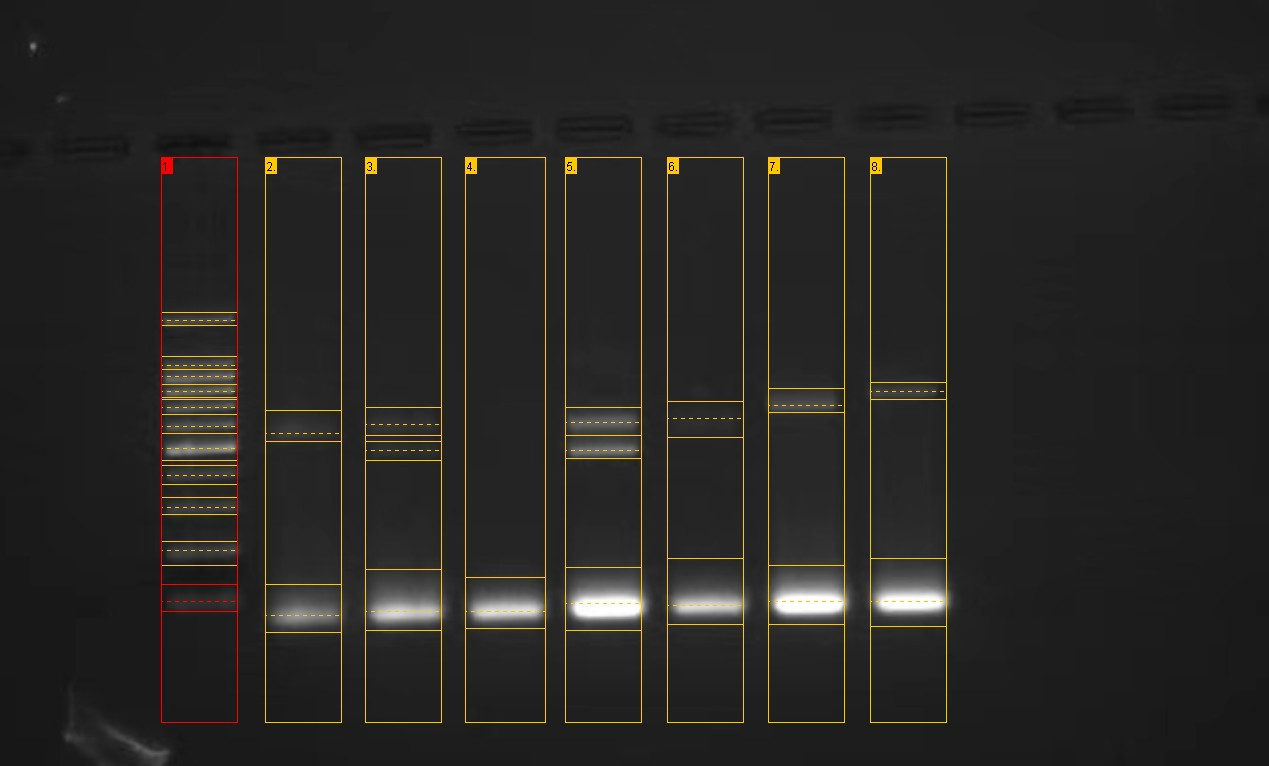
\includegraphics[width=0.4\textwidth]{data/ana_img4-2.jpg}
        \label{fig:anaegimg6}
    }
    \label{fig:anaegimg}
    \caption{电泳分析结果}
\end{figure}

\newpage

\begin{figure}[H]
    \centering

    \hfill
    \subfloat[dataimg1-7]{
        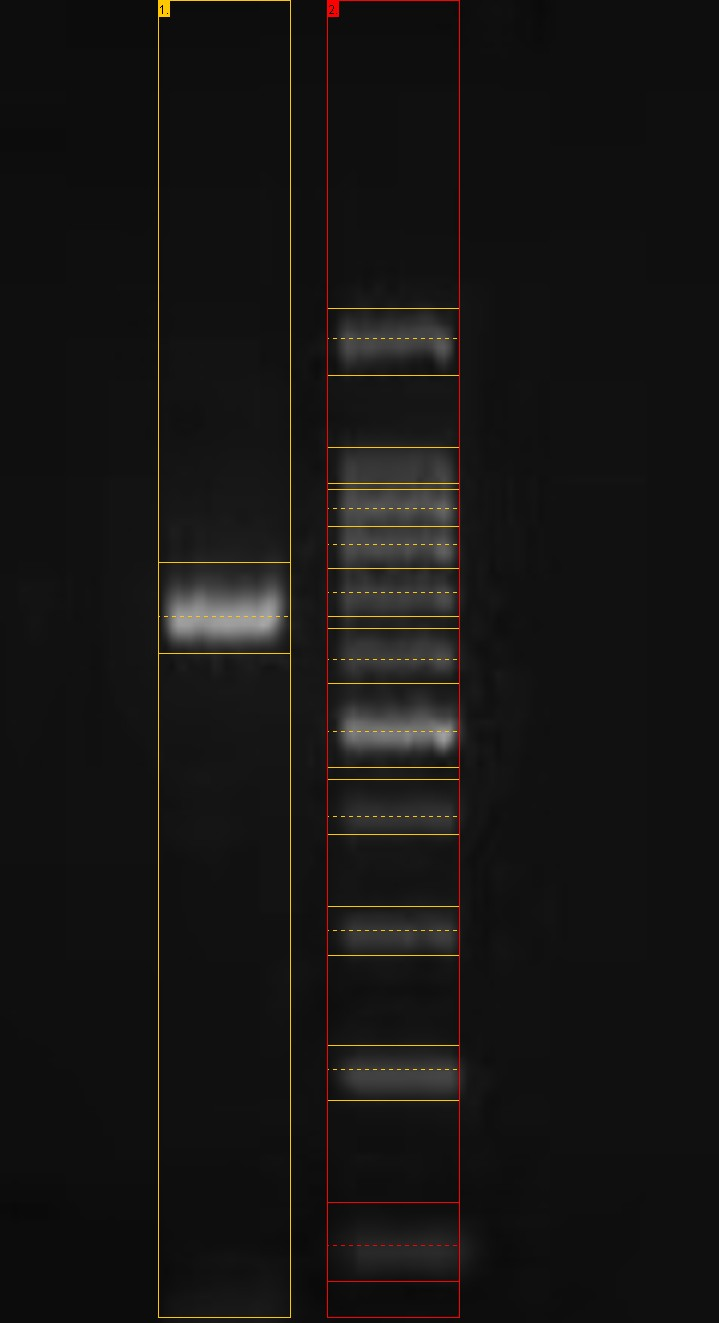
\includegraphics[height=0.3\textwidth]{data/ana_img5-1.jpg}
        \label{fig:anaegimg7}
    }
    \hfill
    \subfloat[dataimg1-8]{
        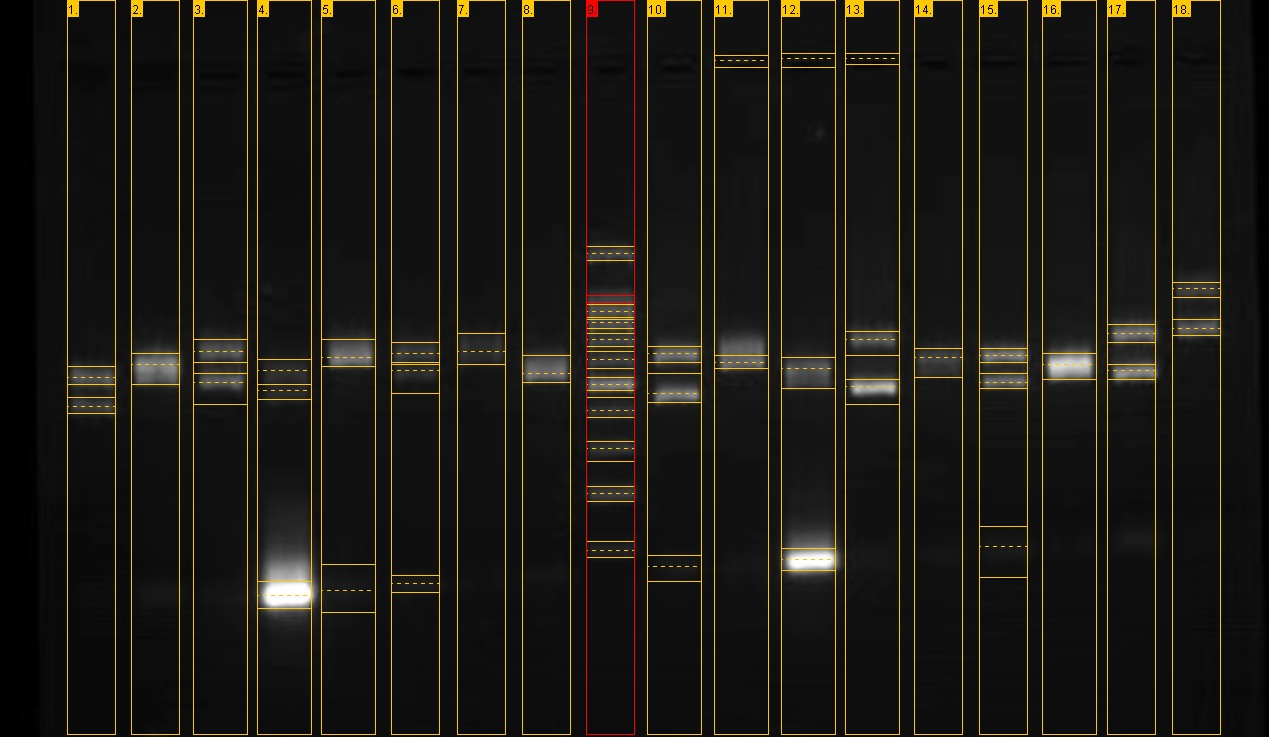
\includegraphics[width=0.4\textwidth]{data/ana_img5-2.jpg}
        \label{fig:anaegimg8}
    }
    \hfill
    \subfloat[dataimg1-9]{
        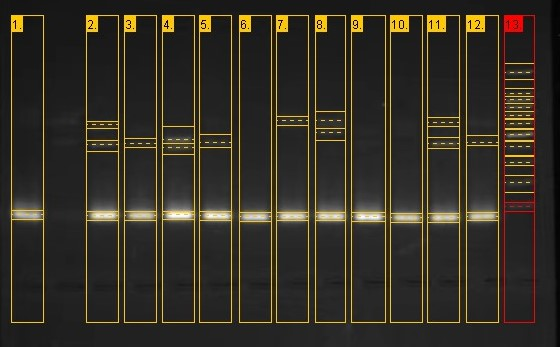
\includegraphics[width=0.4\textwidth]{data/ana_img6-1.jpg}
        \label{fig:anaegimg9}
    }
    \hfill
    \subfloat[dataimg1-10]{
        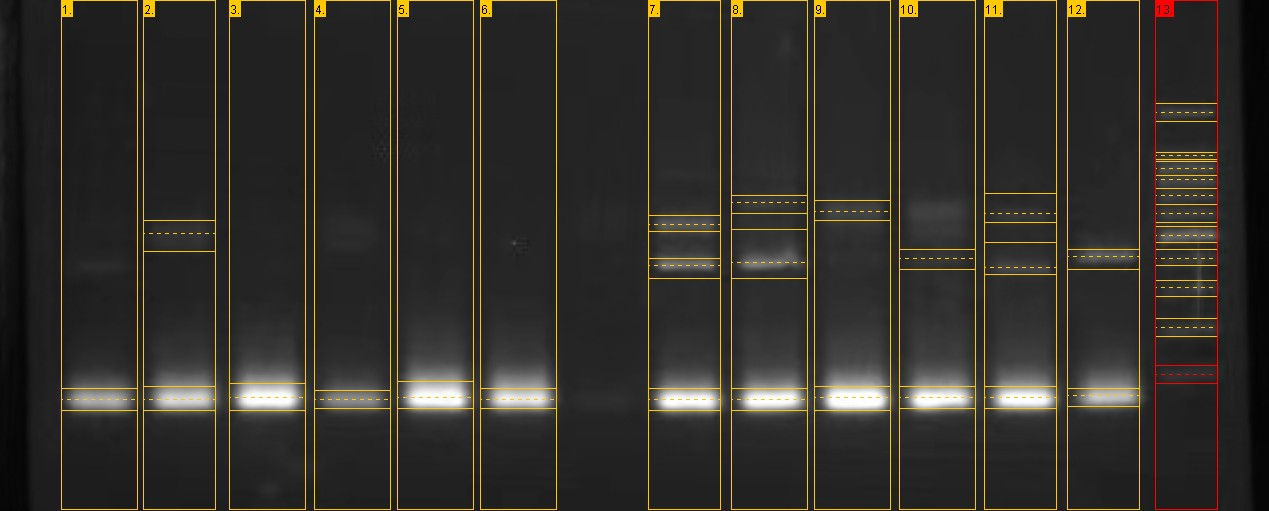
\includegraphics[width=0.4\textwidth]{data/ana_img6-2.jpg}
        \label{fig:anaegimg10}
    }
    \hfill
    \subfloat[dataimg1-11]{
        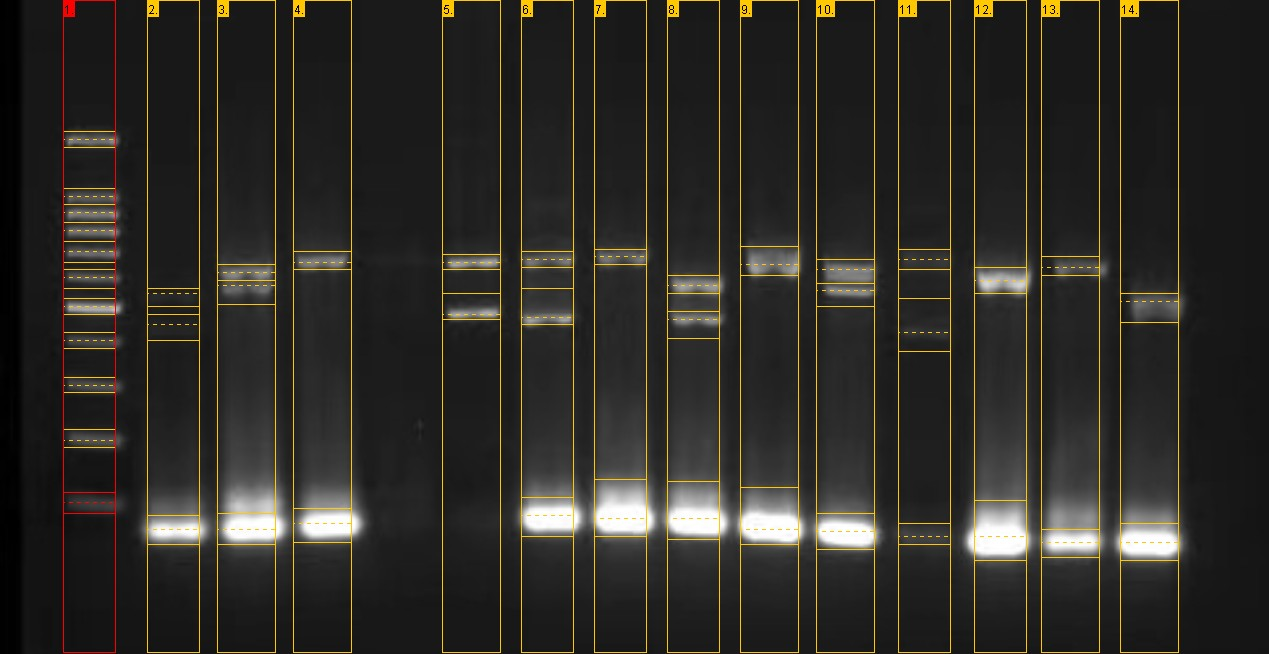
\includegraphics[width=0.4\textwidth]{data/ana_img7-1.jpg}
        \label{fig:anaegimg11}
    }
    \hfill
    \subfloat[dataimg1-12]{
        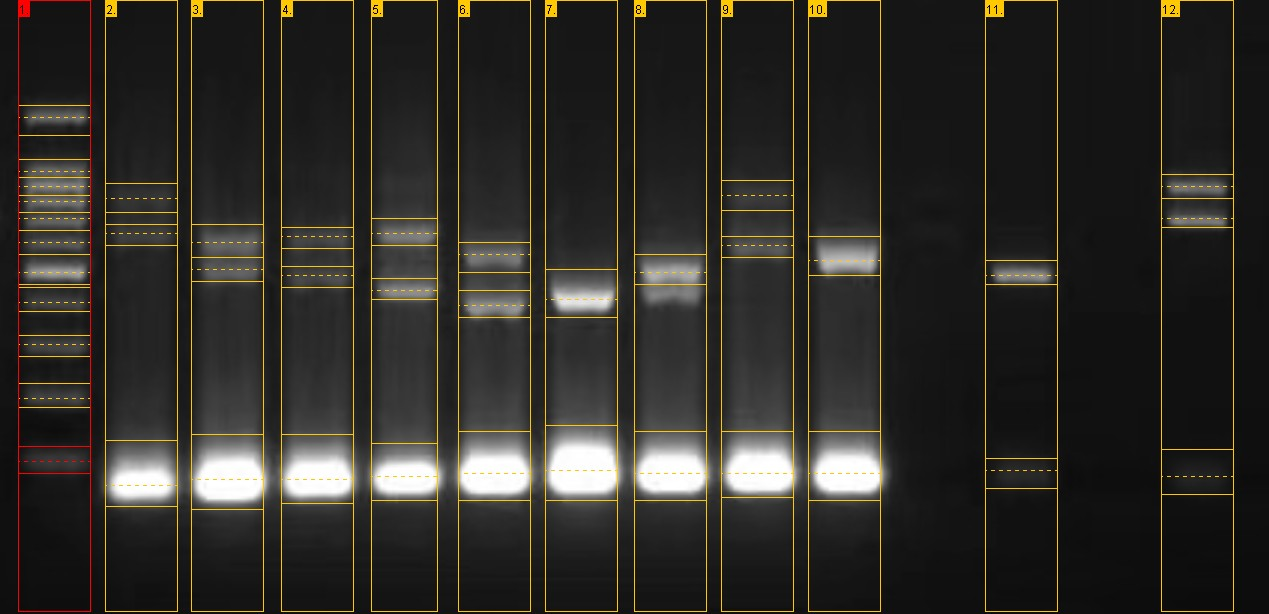
\includegraphics[width=0.4\textwidth]{data/ana_img7-2.jpg}
        \label{fig:anaegimg12}
    }
    \hfill
    \subfloat[dataimg1-13]{
        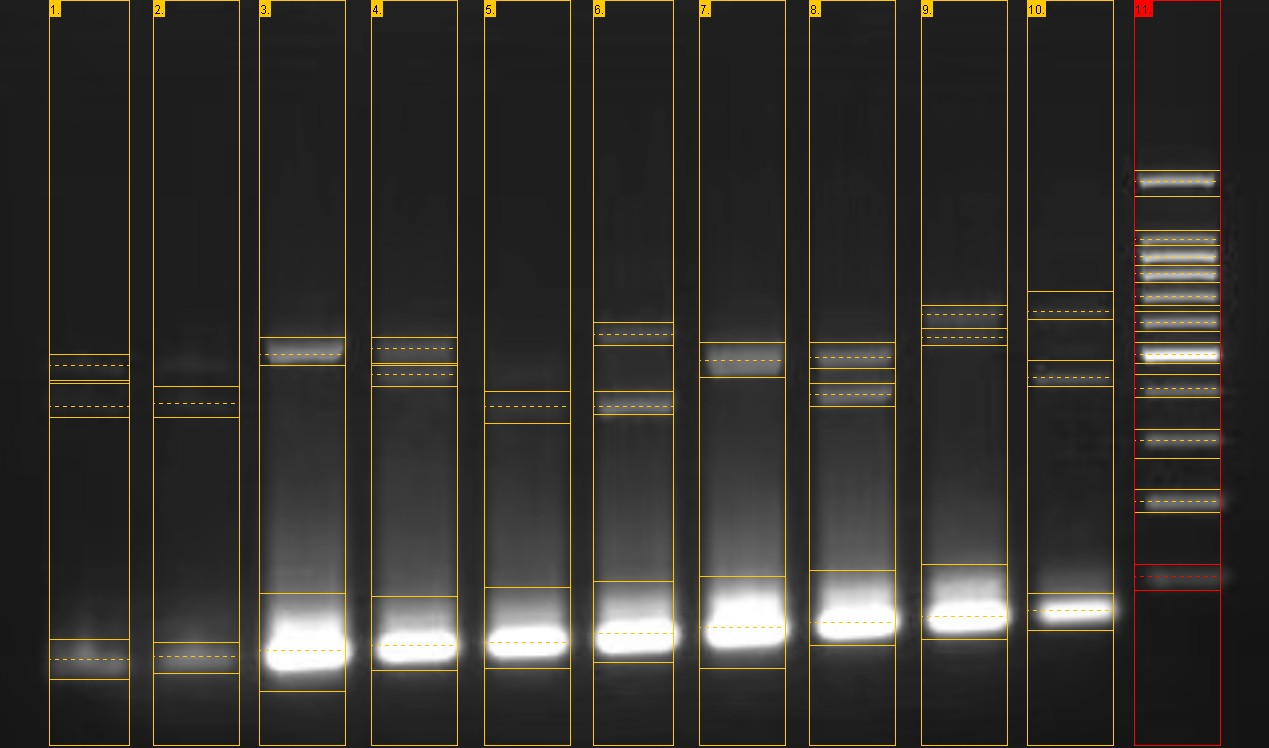
\includegraphics[width=0.4\textwidth]{data/ana_img8-1.jpg}
        \label{fig:anaegimg13}
    }
    \hfill
    \subfloat[dataimg1-14]{
        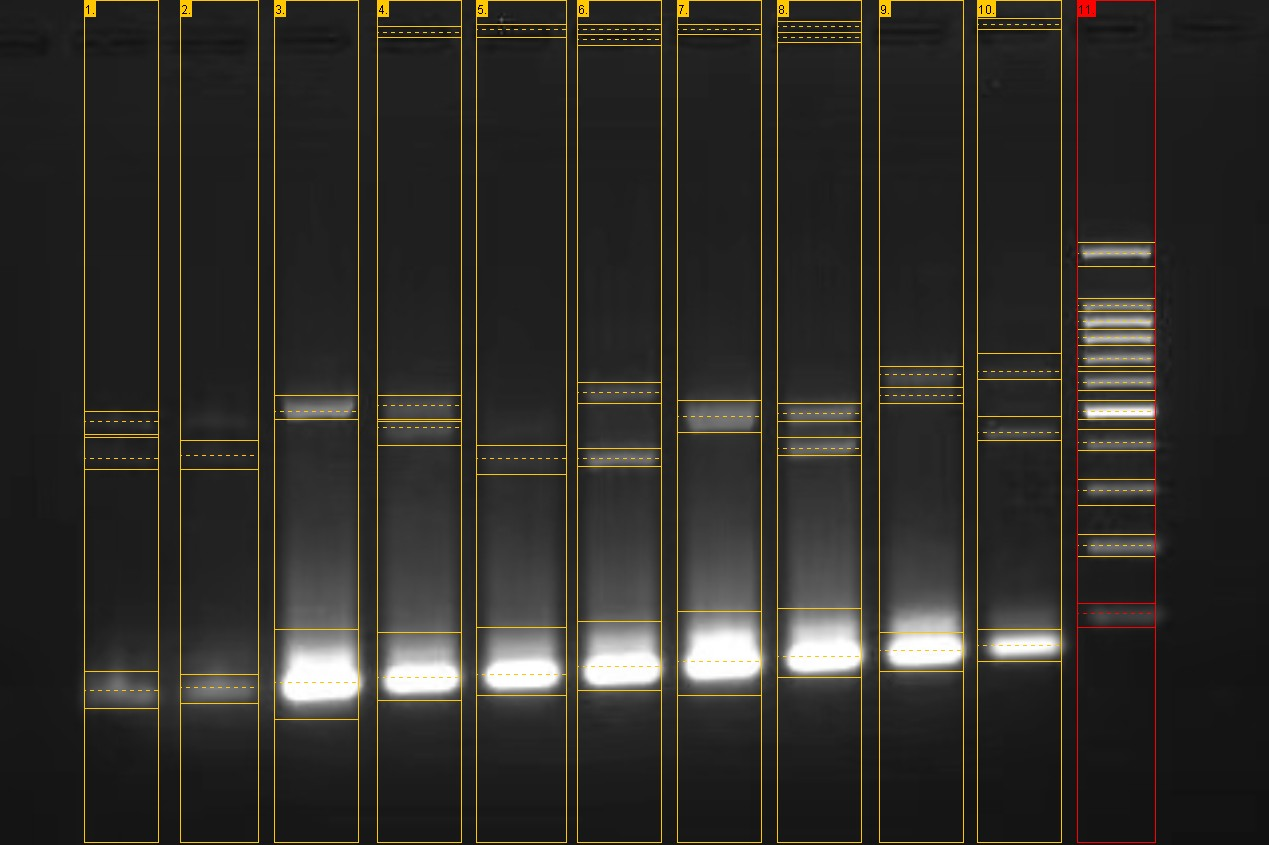
\includegraphics[width=0.4\textwidth]{data/ana_img8-2.jpg}
        \label{fig:anaegimg14}
    }
    \label{fig:anaegimg}
    \caption{电泳分析结果}
\end{figure}    

\newpage


\begin{figure}[H]
    \centering

    \subfloat[dataimg1-15]{
        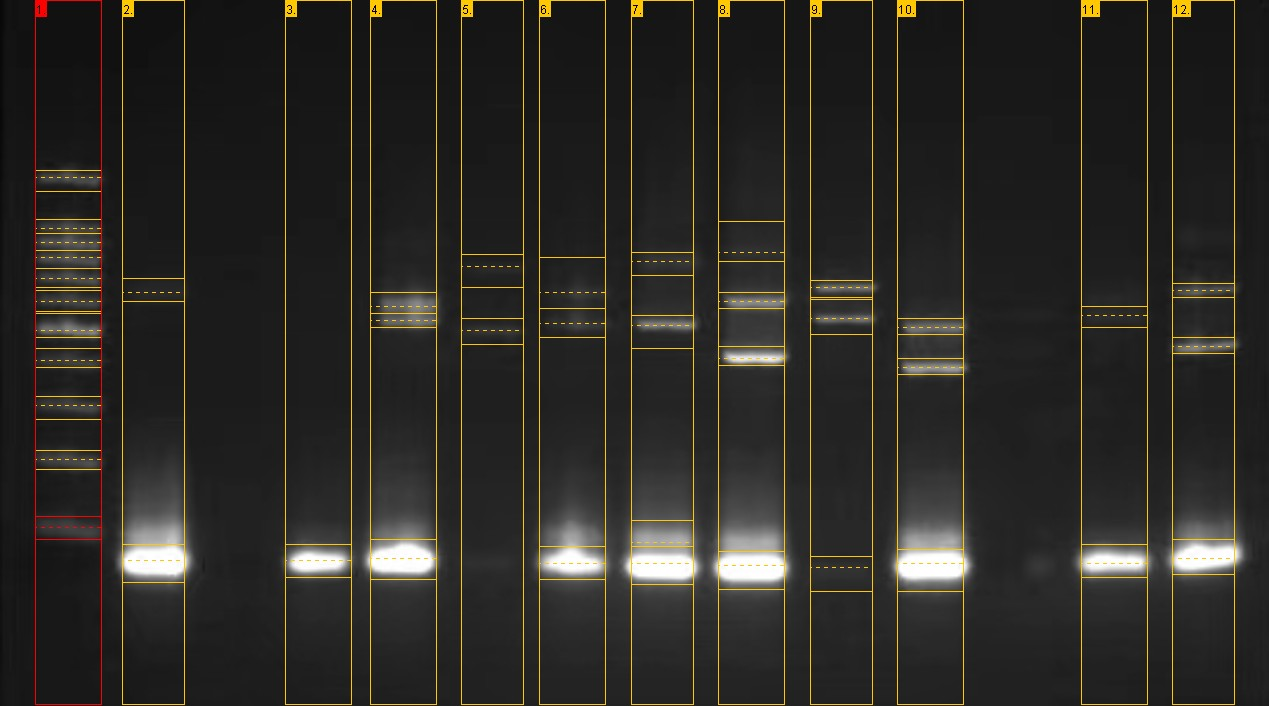
\includegraphics[width=0.4\textwidth]{data/ana_img9-1.jpg}
        \label{fig:anaegimg15}
    }
    \hfill
    \subfloat[dataimg1-16]{
        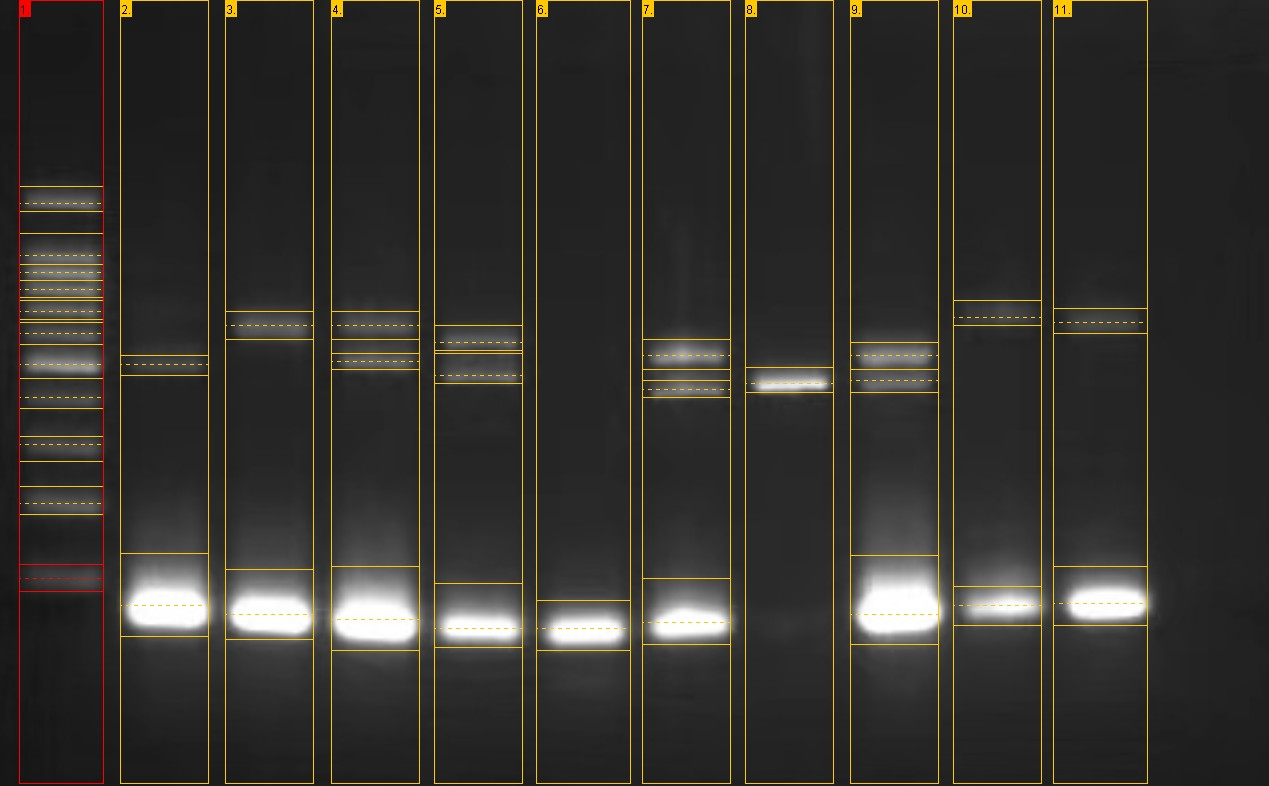
\includegraphics[width=0.4\textwidth]{data/ana_img9-2.jpg}
        \label{fig:anaegimg16}
    }
    \hfill
    \subfloat[dataimg1-17]{
        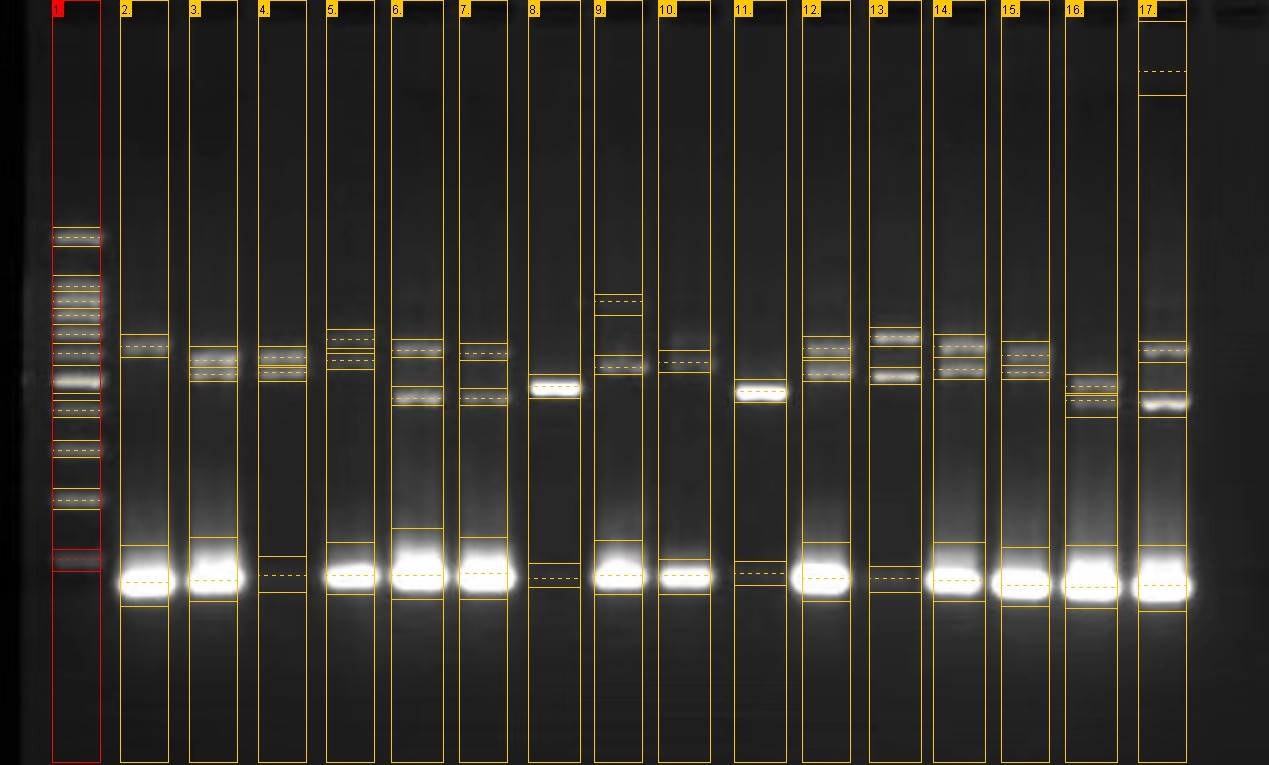
\includegraphics[width=0.4\textwidth]{data/ana_img10-1.jpg}
        \label{fig:anaegimg17}
    }
    \hfill
    \subfloat[dataimg1-18]{
        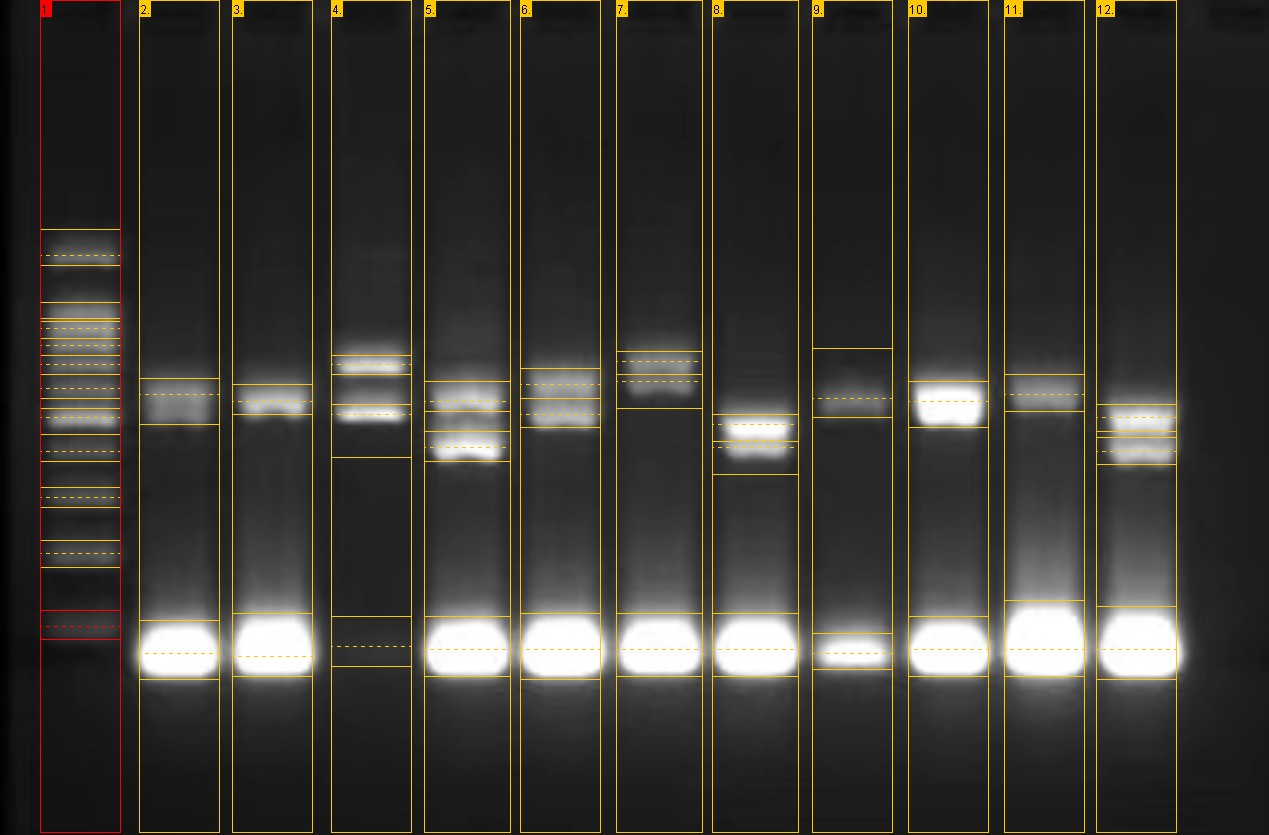
\includegraphics[width=0.4\textwidth]{data/ana_img10-2.jpg}
        \label{fig:anaegimg18}
    }
    
    \label{fig:anaegimg}
    \caption{电泳分析结果}
\end{figure}

\section{重复数总表}

见附录csv文件, 位于/data/summary.csv(\href{https://github.com/zehua0417/GeneticExperimentReport/blob/main/3_Human%20DNA%20Fingerprint%20Analysis/data/summary.csv}{点我打开链接})

\section{数据处理与分析代码}

见附录py文件, 位于/python/main.py(\href{https://github.com/zehua0417/GeneticExperimentReport/blob/main/3_Human%20DNA%20Fingerprint%20Analysis/python/main.py}{点我打开链接})

%\Thanks


%\Grade %这一句才是成绩页,上面是填写


\end{document}
